%%%%%%%%%%%%%%%%%%%%%%%%%%%%%%%%%%%%%%%%%%%%%%%%%%%%%%%%%%%%%%%%%%%%%%%%
%%%  THIS TEX FILE IS TO GENERATE PDF FILE FOR 
%%% 
%%%  COPYRIGHT (C) JIMMY LIN, 2013, UT AUSTIN
%%%%%%%%%%%%%%%%%%%%%%%%%%%%%%%%%%%%%%%%%%%%%%%%%%%%%%%%%%%%%%%%%%%%%%%%
\documentclass[11pt,a4paper]{article}
%%%%%%%%%%%%%%%%%%%%%%%%%%%%%%%%%%%%%%%%%%%%%%%%%%%%%%%%%%%%%%%%%%%%%%%%
%%%  PACKAGES USED IN THIS TEX SOURCE FILE
%%%%%%%%%%%%%%%%%%%%%%%%%%%%%%%%%%%%%%%%%%%%%%%%%%%%%%%%%%%%%%%%%%%%%%%%
\usepackage{geometry,amsthm,amsmath,graphicx,fancyheadings,framed}
\usepackage{tikz}
\usepackage{fancybox}
\usetikzlibrary{automata,positioning}
\usepackage[colorlinks,
            linkcolor=blue,
            anchorcolor=red,
            citecolor=green
            ]{hyperref}
\usepackage{/Users/JimmyLin/workspace/latexTemplate/UTA_CS/JS}
\usepackage{/Users/JimmyLin/workspace/latexTemplate/UTA_CS/JSASGN}
%%%%%%%%%%%%%%%%%%%%%%%%%%%%%%%%%%%%%%%%%%%%%%%%%%%%%%%%%%%%%%%%%%%%%%%%
%%% MACROS CONTAINING THE FILE INFORMATION
%%%%%%%%%%%%%%%%%%%%%%%%%%%%%%%%%%%%%%%%%%%%%%%%%%%%%%%%%%%%%%%%%%%%%%%%
\renewcommand{\COURSE}{CS363D Statistical Learning and Data Mining}
\renewcommand{\LECTURER}{Pradeep Ravikumar}
\renewcommand{\TUTOR}{Adarsh Prasad}
\renewcommand{\TASK}{Homework 01}
\renewcommand{\RELEASEDATE}{Feb. 02 2014}
\renewcommand{\DUEDATE}{Feb. 12 2014}
\renewcommand{\TIMECONSUME}{6 hours}
%%%%%%%%%%%%%%%%%%%%%%%%%%%%%%%%%%%%%%%%%%%%%%%%%%%%%%%%%%%%%%%%%%%%%%%%
%%% DOCUMENTATION STARTS FROM HERE 
%%%%%%%%%%%%%%%%%%%%%%%%%%%%%%%%%%%%%%%%%%%%%%%%%%%%%%%%%%%%%%%%%%%%%%%%
\begin{document}
%%%%%%%%%%%%%%%%%%%%%%%%%%%%%%%%%%%%%%%%%%%%%%%%%%%%%%%%%%%%%%%%%%%%%%%%
%% TITLE PAGE
%%%%%%%%%%%%%%%%%%%%%%%%%%%%%%%%%%%%%%%%%%%%%%%%%%%%%%%%%%%%%%%%%%%%%%%%
\begin{titlepage}
    \maketitle
\end{titlepage}
%%%%%%%%%%%%%%%%%%%%%%%%%%%%%%%%%%%%%%%%%%%%%%%%%%%%%%%%%%%%%%%%%%%%%%%%
%% CONTENT PAGE: TABLEOFCONTENTS, LISTOFTABLES, LIST OF FIGURES
%%%%%%%%%%%%%%%%%%%%%%%%%%%%%%%%%%%%%%%%%%%%%%%%%%%%%%%%%%%%%%%%%%%%%%%%
\renewcommand{\contentsname}{Contents}
\begin{center} 
    \tableofcontents 
    %\listoftables 
    \listoffigures
\end{center}
\newpage
%%%%%%%%%%%%%%%%%%%%%%%%%%%%%%%%%%%%%%%%%%%%%%%%%%%%%%%%%%%%%%%%%%%%%%%%
%%% GENERAL DOCUMENTATION BEGINS 
%%%%%%%%%%%%%%%%%%%%%%%%%%%%%%%%%%%%%%%%%%%%%%%%%%%%%%%%%%%%%%%%%%%%%%%%

\section{Jaccard Distance}
\newcommand{\M}[1]{\ensuremath{M_{#1}}}
\newcommand{\binEpy}[2]{\ensuremath{-\big( \frac{#1}{#2} log_2(\frac{#1}{#2}) 
+ \frac{#2-#1}{#2} log_2(\frac{#2-#1}{#2})\big)}}

\ovalbox{
    \begin{minipage}{16.5cm}
Consider two binary vectors $\mathbf{u}$ and $\mathbf{v}$. Suppose the total
number of ones in both the binary vectors together is $n$; and that dot
product of the two vectors is $d$. What is the Jaccard distance between
$\mathbf{u}$ and $\mathbf{v}$?
\end{minipage}
}
\\

According to the Jaccard terminology for measuring the similarity of two
vectors, $\M{11}$ represents the number of dimensions where both vectors has
value 1 and $\M{10} + \M{01}$ represents the number of dimensions where either
vectors has value 1.

Since for given two binary vector $\mathbf{u}$ and $\mathbf{v}$, total number
of ones in both the binary vectors together is $n$, and dot product of the two
vectors is $d$, we have
\begin{align*}
    \M{11} &= d \\
    \M{10} + \M{01} &= n-2d 
\end{align*}
Note that the dot product only count the dimensions where both vectors are 1.
\\

By the definition of Jaccard Distance, we have
\begin{align*}
    J &= \frac{\M{00}}{\M{01} + \M{10} + \M{11}} \\
      &= \frac{d}{n-2d+d} \\
      &= \frac{d}{n-d}
\end{align*}

Thus, the Jaccard Distance between $\mathbf{u}$ and $\mathbf{v}$ is
$\frac{d}{n-d}$.

\newpage 

\section{Binary Classification Data Set}
\newcommand{\dtnode}[3]{\ensuremath{#1, (#2,#3)}}
Consider the binary classification data set, with two attributes A and B. \\

\textbf{Split on attribute A:} 

\begin{figure}[h]
    \centering
\ovalbox{
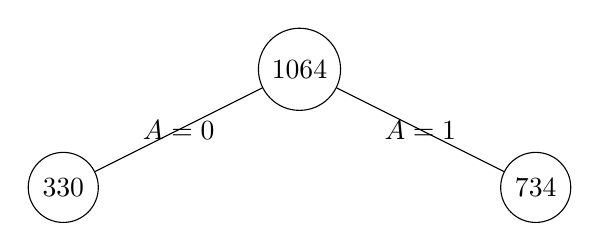
\begin{tikzpicture}[level/.style={sibling distance=60mm/#1}]
    \node [circle,draw] (root){$\dtnode{10}{6}{4}$}
    child {node [circle,draw] (a) {$\dtnode{3}{3}{0}$} }
    child {node [circle,draw] (b) {$\dtnode{7}{3}{4}$} }
    ;
    \path (root) -- (a) node [midway] {$A=0$};
    \path (root) -- (b) node [midway] {$A=1$};
\end{tikzpicture}
}
\caption{Decision Tree split on attribute A}
\end{figure}

\textbf{Split on attribute B:} 

\begin{figure}[h]
    \centering
\ovalbox{
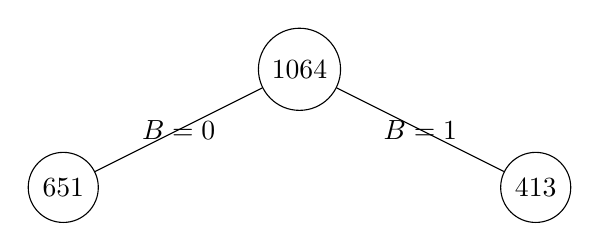
\begin{tikzpicture}[level/.style={sibling distance=60mm/#1}]
    \node [circle,draw] (root) {$\dtnode{10}{6}{4}$}
    child {node [circle,draw] (a) {$\dtnode{6}{5}{1}$}}
    child {node [circle,draw] (b) {$\dtnode{4}{1}{3}$}}
    ;
    \path (root) -- (a) node [midway] {$B=0$};
    \path (root) -- (b) node [midway] {$B=1$};
\end{tikzpicture}
}
\caption{Decision Tree split on attribute B}
\end{figure}

Note that for $N, (A, B)$ in each node,
\begin{center}
    N represents number of records in that nodes \\
    A represents number of records with class "+" \\
    B represents number of records with class "-"  
\end{center}

\newpage
\subsection{Gain in Gini index} 

\ovalbox{
    \begin{minipage}{16.5cm}
Calculate the gain in Gini index when splitting on A and B. Which attribute
would the decision tree induction algorithm choose?
Now let us look at the decision tree split by attribute A and attribute B. 
\end{minipage}
}
\\

The computation of Gini index split by attribute A is as follows:
\begin{align*}
    Gini(root) &= 1 - (\frac{6}{10})^2 - (\frac{4}{10})^2 = 0.48 \\
    Gini(leftChild) &= 1 - (\frac{3}{3})^2 - (\frac{0}{3})^2 = 0 \\
    Gini(rightChild) &= 1 - (\frac{3}{7})^2 - (\frac{4}{7})^2 = 0.490 
 \end{align*}

 Thus, the gain of Gini index by spliting at attribute A $Gain_A$ is 
\begin{align*}
    Gain_A &= Gini(root) - \frac{3}{10} Gini(leftChild) - \frac{7}{10}Gini(rightChild) \\
           &= 0.48 - \frac{7}{10} \times 0.49  = 0.137
 \end{align*}

The computation of Gini index split by attribute B is as follows:
\begin{align*}
    Gini(root) &= 1 - (\frac{6}{10})^2 - (\frac{4}{10})^2 = 0.48 \\
    Gini(leftChild) &= 1 - (\frac{5}{6})^2 - (\frac{1}{6})^2 = 0.278 \\
    Gini(rightChild) &= 1 - (\frac{1}{4})^2 - (\frac{3}{4})^2 = 0.375 
 \end{align*}

 Thus, the gain of Gini index by spliting at attribute B $Gain_B$ is 
\begin{align*}
    Gain_B &= Gini(root) - Gini(leftChild) - Gini(rightChild) \\
           &= 0.48 - \frac{6}{10} \times 0.278 - \frac{4}{10} \times 0.375 =
    0.1632
 \end{align*}

  Comparing the gain of Gini index $Gain_A$ and $Gain_B$, we have

 $$
        Gain_A < Gain_B
 $$

 Thus, \textbf{attribute B} is the one we should choose to split since it maximize the
Gini gain.

\newpage
\subsection{Information Gain}
\ovalbox{
    \begin{minipage}{16.5cm}
Repeat part (a) with information gain (i.e. gain in the entropy measure). \\
\end{minipage}
}
\\

The computation of Entropy split by attribute A is as follows:
\begin{align*}
    Entropy(root) &= \binEpy{6}{10} = 0.971 \\
    Entropy(leftChild) &= \binEpy{3}{3} = 0 \\
    Entropy(rightChild) &= \binEpy{3}{7} = 0.985 
 \end{align*}

 Thus, the Information Gain by spliting at attribute A $Gain_A$ is 
\begin{align*}
    IGain_A^* &=  Entropy(root)- \frac{3}{10}Entropy(leftChild) - \frac{7}{10} Entropy(rightChild) \\
        &= 0.971 - 0 - \frac{7}{10} * 0.985 = 0.2815
 \end{align*}

The computation of Entropy split by attribute B is as follows:
\begin{align*}
    Entropy(root) &= \binEpy{6}{10} = 0.971 \\
    Entropy(leftChild) &= \binEpy{5}{6} = 0.65 \\
    Entropy(rightChild) &= \binEpy{1}{4} = 0.811 
 \end{align*}

 Thus, the Information Gain by spliting at attribute B $Gain_B$ is 
\begin{align*}
    IGain_B^{*} &= Entropy(root) - \frac{6}{10} Entropy(leftChild) -
    \frac{4}{10}Entropy(rightChild) \\
    &= 0.971 - \frac{6}{10} * 0.65 - \frac{4}{10} * 0.811 = 0.2566 
 \end{align*}

 Comparing the gain of Gini index $IGain_A$ and $IGain_B$, we have

 $$
    IGain_A > IGain_B
 $$

 Thus, \textbf{attribute A} is the one we should choose to split since it maximize the
Information gain.

\newpage

\section{Decision Tree}
\ovalbox{
    \begin{minipage}{16.5cm}
Compute a two-level decision tree for the training data using the
greedy approach discussed in the class, with gain in Gini index as the
criterion for splitting. What is the overall error rate on the training data
of the induced tree?
\end{minipage}
}
\\
\begin{figure}[h]
    \centering
    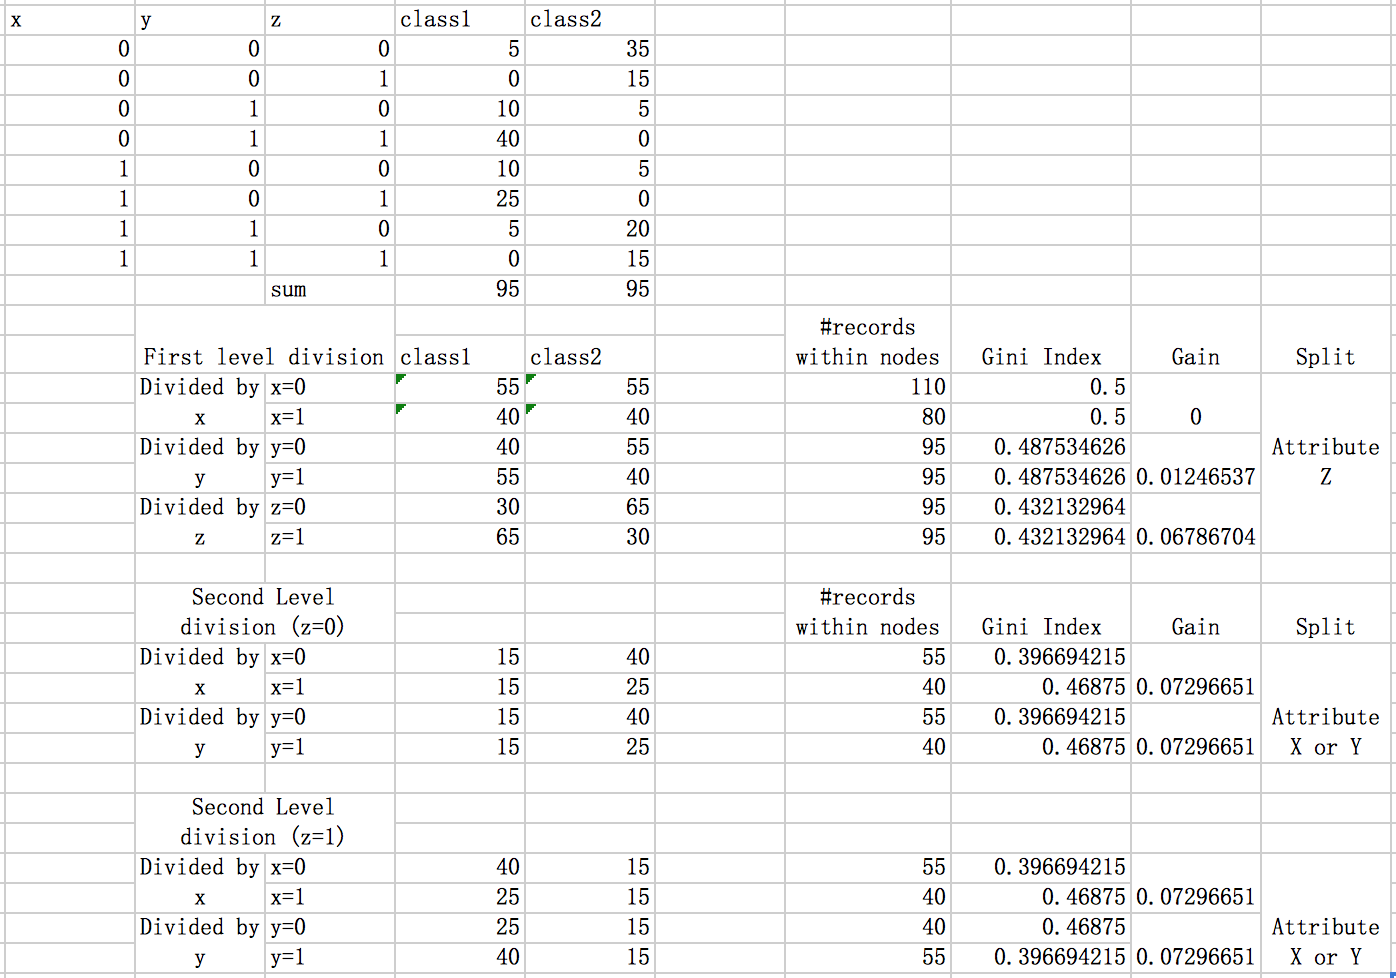
\includegraphics[width=5in,height=4in]{./section3.png} \\
    \caption{Statistics about the decision tree production}
\end{figure}

Construction of decision tree is simple. The technique we employ here is to
evaluate whether the class distribution derived by candidate division is close
to uniform distribution. According to this principle, we expand over attribute
$z$ at the root node and afterwards we can either expand over attribute $x$ or
$y$ on both branches of $z=0$ and $z=1$.  

The resulted decision tree (just one possile solution) is as follows:

\begin{figure}[h]
    \centering
\ovalbox{
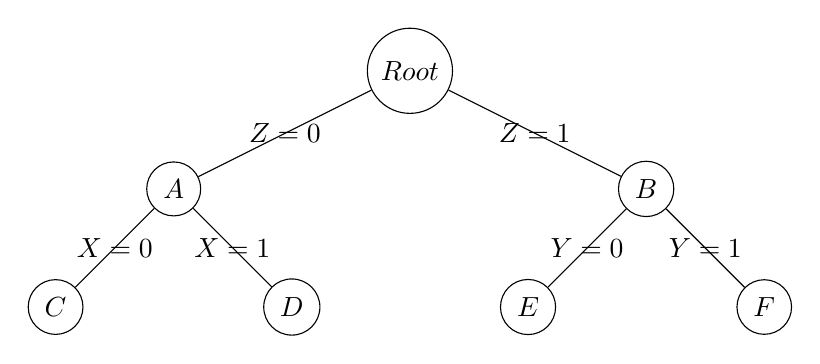
\begin{tikzpicture}[level/.style={sibling distance=60mm/#1}]
    \node [circle,draw] (root){$Root$}
    child {node [circle,draw] (a) {$A$} 
        child {node [circle,draw] (c) {$C$} }
        child {node [circle,draw] (d) {$D$} }
    }
    child {node [circle,draw] (b) {$B$}
        child {node [circle,draw] (e) {$E$} }
        child {node [circle,draw] (f) {$F$} }
    }
    ;
    \path (root) -- (a) node [midway] {$Z=0$};
    \path (root) -- (b) node [midway] {$Z=1$};
    \path (a) -- (c) node [midway] {$X=0$};
    \path (a) -- (d) node [midway] {$X=1$};
    \path (b) -- (e) node [midway] {$Y=0$};
    \path (b) -- (f) node [midway] {$Y=1$};
\end{tikzpicture}
}
\caption{Constructed Decision Tree}
\end{figure}

For this instance, we classify all records in C and D as "class 1" object, and
in the meanwhile assign all records in E and F as "class 2" object. Thus, the training
error rate $e$ would be 
    $$
    e = (30 + 30) / 190 = 31.58\%
    $$

%%%%%%%%%%%%%%%%%%%%%%%%%%%%%%%%%%%%%%%%%%%%%%%%%%%%%%%%%%%%%%%%%%%%%%%%
%%% General Documentation ends
%%%%%%%%%%%%%%%%%%%%%%%%%%%%%%%%%%%%%%%%%%%%%%%%%%%%%%%%%%%%%%%%%%%%%%%%
\end{document}
